
\documentclass[preprint,12pt]{elsarticle}

\usepackage[spanish]{babel}
\usepackage{amssymb}
\usepackage{graphicx}
\usepackage{lineno}
\usepackage[utf8]{inputenc}
\usepackage{url}
\usepackage{color}



\begin{document}
	
	\begin{frontmatter}
		
		
		\title{\huge Balanced ScoreCard vs Business Model Canvas}
		
		\author{Mamani Ayala, Brandon        (2015052715)}
		\author{Quispe Mamani, Angelo	      (2015052826)}
		\author{Vizcarra Llanque, Jhordy	      (2015052719)}
		\author{Ordoñez Quilli, Ronald          (2015052821)}
		\author{Rodriguez Mamani, Juan      (2017057862)}
		
		\address{Tacna, Perú}
		
		\begin{abstract}
			%% Text of abstract
			Performance Management bevat activiteiten die ervoor kunnen zorgen dat doelen consistent worden behaald op een effectieve en efficiënte wijze. Middels het Business Model Canvas wordt u een concept aangeboden, waarmee u het business model van uw organisatie kunt beschrijven, overdenken en onderzoeken. Een business model kan het beste worden beschreven aan de hand van negen basisbouwstenen, die de logica laten zien van hoe een bedrijf geld wil gaan verdienen.
Na een strategische heroriëntatie in een snel veranderende omgeving, gaan wij verder in op de best practice in performance management, de Business Balanced Scorecard (‘BSC’). De nadruk ligt op de praktische implementatie van de BSC en het bouwen van een gebalanceerde dashboard, waarbij niet alleen rekening wordt gehouden met een financial dashboard, maar ook met het klantperspectief, intern en innovatief perspectief.
	
		\end{abstract}
\end{frontmatter}
%%

	
	%%
	%\linenumbers
	
	%% main text
	
	%%
	%\linenumbers
	
	%% main text



\section{Balanced ScoreCard }

\title{Balanced Scorecard}
El Balanced Scorecard (BSC / Cuadro de Mando Integral) es una herramienta que permite enlazar estrategias y objetivos clave con desempeño y resultados a través de cuatro áreas críticas en cualquier empresa: desempeño financiero, conocimiento del cliente, procesos internos de negocio y aprendizaje y crecimiento. \\
Sin embargo, es algo más que un nuevo sistema de medición. Las empresas innovadoras utilizan el Cuadro de Mando integral como el marco y estructura central y organizativa para sus procesos. Las empresas pueden desarrollar un Cuadro de mando Integral, con unos objetivos bastante limitados: conseguir clarificar, obtener el consenso y centrarse en su estrategia, y luego comunicar esa estrategia a toda la organización. Sin embargo, el verdadero poder del Cuadro de mando Integral aparece cuando se transforma de un sistema de indicadores en un sistema de gestión. A medida que más y más empresas trabajan con el 
Cuadro de Mando Integral, se dan cuenta de que puede utilizarse para:
		\begin{itemize}
		\item Clarificar la estrategia y conseguir el consenso sobre ella.
		\item Comunicar la estrategia a toda la organización.
		\item Alinear los objetivos personales y departamentales con la estrategia.
		\item Vincular los objetivos estratégicos con los objetivos a largo plazo y los presupuestos anuales.
		\item Identificar y alinear las iniciativas estratégicas.
		\item Realizar revisiones estratégicas periódicas y sistemáticas
		\item Obtener feedback para aprender sobre la estrategia y mejorarla.
		\end{itemize}

\begin{center}
	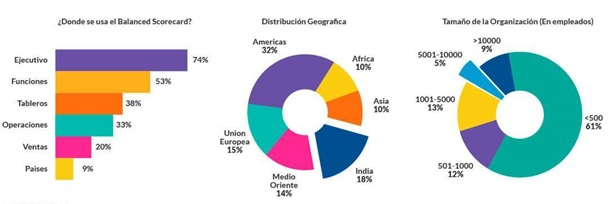
\includegraphics[width=12cm]{./Imagenes/img1} 
\end{center}

El cuadro de mando integral llena el vacío que existe en la mayoría de sistemas de gestión: la falta de un proceso sistemático para poner en práctica la estrategia y obtener feedback sobre ella. Los procesos de gestión alrededor del Cuadro de Mando permiten que la organización se equipare y se centre en la puesta en práctica de la estrategia a largo plazo. Utilizado de este modo, el Cuadro de Mando Integeral se convierte en los cimientos para gestionar las organizaciones de la era de la información.\\
\\
En la siguiente figura se presentan las cuatro perspectivas del Cuadro de Mando Integral, se puede apreciar que es un sistema que considera todos los procesos estratégicos de la organización:

\begin{center}
	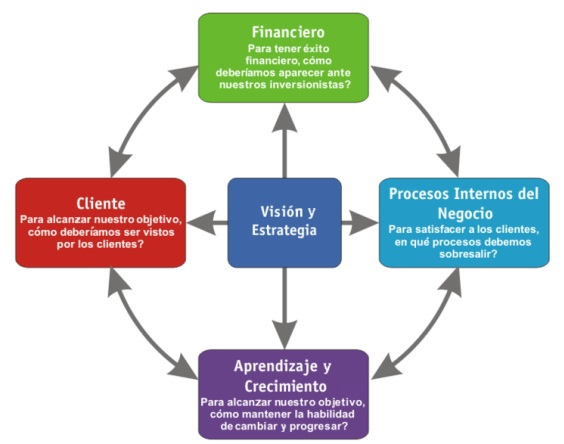
\includegraphics[width=10cm]{./Imagenes/img2} 
\end{center}

Balanced Scorecard, ejemplo de mapa estratégico de una joyería

\begin{center}
	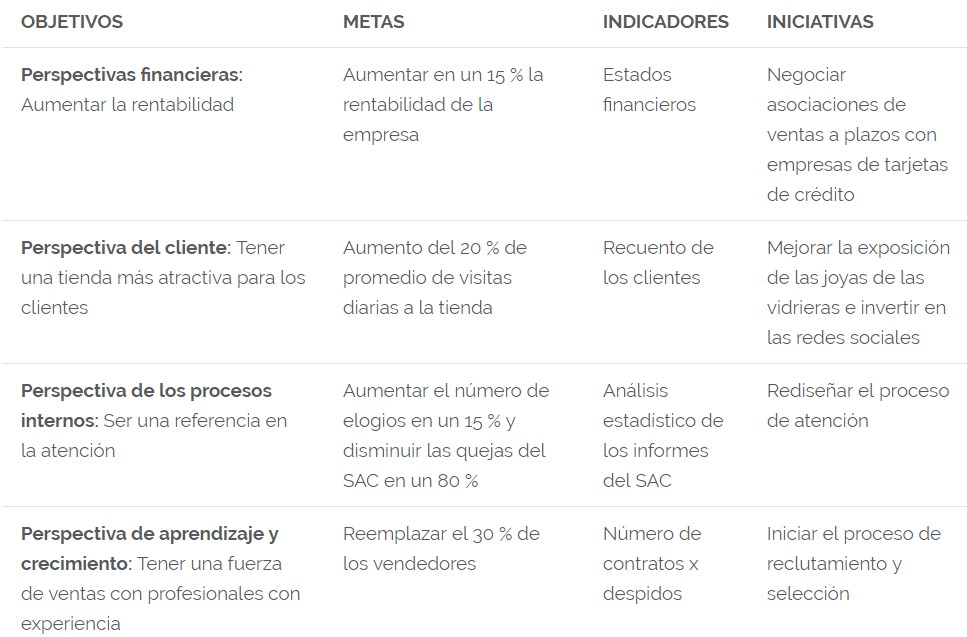
\includegraphics[width=13cm]{./Imagenes/img3} 
\end{center}

Areas críticas de Balanced Scorecard:
		\begin{itemize}
		\item Indicadores desde la perspectiva de los procesos internos: Desde esta perspectiva son analizados aquellos procesos de la empresa que están dirigidos a obtener el rendimiento esperado en los tiempos programados. Así, este grupo de indicadores incluye aquellos que están relacionados con la calidad del proceso, como son los indicadores de productividad, de calidad del producto, de costos del producto, de eficiencia del proceso de fabricación.

Igualmente, serán considerados en este grupo los indicadores de tiempos de entrega, de calidad de materias primas, de mantenimiento de productos, así como los indicadores medioambientales.
		\item Indicadores desde la perspectiva del cliente: En este grupo se encuentran los indicadores relacionados con las soluciones destinadas a satisfacer las necesidades de los clientes. También se consideran aquellos vinculados a mejorar la cuota de mercado de la empresa.

Entre dichos indicadores se encuentran la fidelidad del cliente, la satisfacción del cliente, la calidad  que se percibe de nuestro producto o servicio, la imagen que los clientes tienen de la empresa, la calidad del servicio postventa y del servicio de atención al cliente.

		\item Indicadores desde la perspectiva financiera: Aquí se consideran los indicadores analizados desde la contabilidad y las finanzas, especialmente aquellos que dan cuenta de la situación económica de la empresa. Entre dichos indicadores podemos considerar las ampliaciones de capital, las fusiones o absorciones, la emisión de acciones, bonos u otros instrumentos financieros y la creación de filiales.

También integran este grupo de indicadores la gestión del riesgo, la liquidez de la empresa, el endeudamiento, etc.

		\item Indicadores desde la perspectiva de la innovación y aprendizaje: En este cuarto grupo de indicadores se considera aquellos relacionados con la introducción de innovación en los diversos procesos de la organización, la capacitación de los trabajadores, ventas por lanzamiento de nuevos productos o servicios, ahorros de costos por innovación en procesos, ROI por la inversión en innovación, ratio de éxito de nuevos productos, incremento de capacidades en el personal, etc.

La implementación y análisis de estos indicadores en la forma de cuadro de mando integral permitirá realizar el control de diversos aspectos estratégicos de la organización, lo cual llevará a tomar decisiones relacionadas con acciones preventivas y correctivas, así como de mejoramiento del rendimiento mediante la implementación de las cuatro perspectivas señaladas.
	\end{itemize}


Ventajas de Balanced Scorecard:
\begin{itemize}
		\item Permite tener una visión y control de cómo el funcionamiento de cada área y miembro de la empresa influye en el resto de la organización.
		\item Establecer una vinculación entre los objetivos de la empresa y las acciones necesarias para lograrlos.
		\item Una vez ejecutadas las acciones de mejora, detectar cómo influyen en otras áreas de la empresa, lo que permitirá ejecutar correcciones adicionales si es necesario.
		\item Implantar un modelo de gestión flexible e interactivo, acorde a los actuales requerimientos y exigencias del mercado.
		\item Incorporación de perspectivas distintas a las financieras, como la perspectiva del cliente o la interna o de procesos de negocio.
		\item Disponer de una una imagen muy clara y gráfica del status de la organización en cada momento en cuanto a metas, resultados y acciones en desarrollo o ya implantadas.
		\item Ayuda a tomar las decisiones más acertadas en el momento oportuno para maximizar la rentabilidad y productividad de la empresa.
		\item Facilita la comunicación entre dirección, mandos intermedios y empleados para que todos tenga una idea muy clara de los objetivos, específicos y generales, de la empresa y de las acciones necesarias para lograrlos.
	\end{itemize}


	%%
	
	%%
	%\linenumbers
	
	%% main text
\pagebreak

\section{Business Model Canvas}
	
\subsection{¿Qué es el Business Model Canvas?}	
Es una herramienta nueva, que hace unos años (2010) vio la luz gracias al libro  “Generación de modelos de negocio” (Business Model Generation) escrito por Alex Osterwalder e Yves Pigneur. Este libro se caracteriza por ser una guía para visionarios, revolucionarios y retadores que quieren desafiar los anticuados modelos de negocio y diseñar las empresas del futuro. \\
Cuenta con nueve módulos que forman parte del método canvas, aunque se podrían dividir en 4 áreas diferentes los cuales son:\\
\begin{enumerate}[1.]
\item La oferta.
\item Los clientes.
\item La estructura.
\item La viabilidad económica del proyecto.

	\begin{center}
	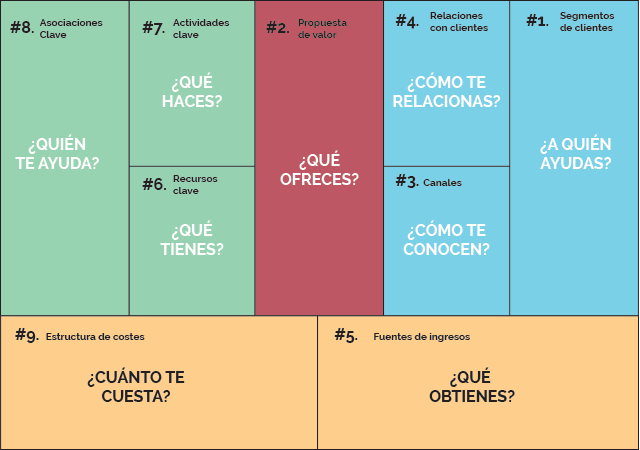
\includegraphics[width=13cm]{./Imagenes/canvas}
	\end{center}

\end{enumerate}
\pagebreak

\subsection{Beneficios del modelo canvas para tu negocio}
\begin{itemize}	
\item La principal ventaja del canvas model es la sencillez con la que se puede trabajar a la hora de definir un modelo de negocio.
\item Uno de los principales beneficios del lienzo de canvas es que podemos ver de una forma muy visual los elementos más importantes del modelo de negocio de una organización.
\item Nos permite también una mayor adaptación al cambio. La metodología canvas se basa en tratar de adaptar tu modelo de negocio a los cambios que se van produciendo en el entorno y en la propia empresa. Al ver los elementos más importantes de la organización de una forma integral, puede ser más sencillo determinar qué elementos están fallando en la consecución de los objetivos.
\item Otra de las ventajas de adoptar la metodología canvas es que permite trabajar en equipo.
\end{itemize}

\subsection{Elementos que forman parte del Business Model Canvas}

\subsubsection{Segmentos de Clientes}
Los clientes deben de ser el centro de cualquier tipo de negocio, como se suele decir, son la razón de ser de una organización.
Da igual la propuesta de valor que tenga tu empresa, que si no satisface las necesidades de ningún segmento de clientes, tu negocio estará destinado al fracaso.	
	\begin{center}
	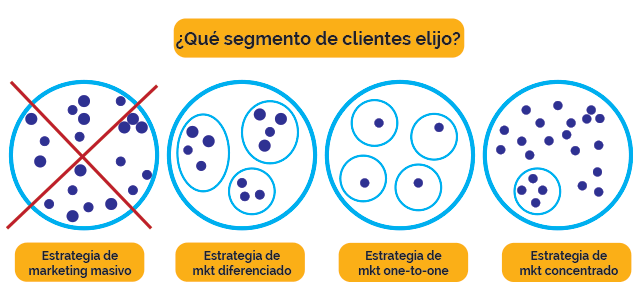
\includegraphics[width=13cm]{./Imagenes/canvas1}
	\end{center}
Tener claro cómo definir tu público objetivo puede marcar el éxito o el fracaso de un proyecto.
Los clientes no se tienen que adaptar a tu propuesta de valor, eres tú quien debes de adaptar la propuesta de valor de tu negocio a sus necesidades y deseos.
Por lo que el primer paso será tener claro a qué segmento de clientes te quieres dirigir.\\
Alguna de las preguntas que te puedes hacer y que te ayudarán a definir a tu cliente ideal pueden ser:\\
\begin{itemize}
\item ¿Por qué les pueden interesar mis productos?
\item ¿Qué tipo de producto es más adecuado para cada segmento?
\item ¿Qué diferencia mi propuesta de valor de la del resto de competidores?
\item ¿Qué les podría impedir comprar mis productos?
\item ¿Cuáles son sus deseos, sus metas y sus motivaciones?
\item ¿Con qué canales tendríamos más fácil llegar a ellos?
\end{itemize}

\subsubsection{Propuesta de Valor}
El segundo punto de tu modelo de negocio canvas será la propuesta de valor de tu negocio.
La propuesta de valor de una empresa y el segmento de clientes son la base cualquier modelo de negocio
La propuesta de valor hay que entenderla como el conjunto de beneficios que le vamos a aportar a nuestros clientes con nuestros productos y servicios.
Es la razón por la que los clientes nos elegirán a nosotros como alternativa en lugar de a la competencia.
Hay que diseñarla en función de las necesidades del cliente pero también fijar un precio que esté dispuesto a pagar y que sea rentable para nuestro negocio.\\
Aquí es fundamental conocer:\\
\begin{itemize}
\item ¿Qué problema ayudamos a solucionar?
\item ¿Qué valor diferencial ofrecemos a nuestros clientes?
\end{itemize}
Por ejemplo, en el libro de Generación de Modelos de Negocio, recoge que los principales elementos para ofrecer un valor diferencial son:\\
\begin{enumerate}[1.]
\item Precio
\item Novedad
\item Calidad
\item Conveniencia
\item Marca o Status
\item Desempeño
\item Reducción de riesgo
\item Reducción de costes
\item Diseño
\item Customización
\end{enumerate}
A la hora de crear tu business canvas model lo que deberás de hacer es elegir aquellos factores que te van a permitir diferenciarte y buscar una posición competitiva ventajosa en tu nicho de mercado.

\subsubsection{Canales}
¿De qué sirve tener la mejor propuesta de valor y una demanda de mercado si no tenemos los canales adecuados?
Es en este punto dónde vamos a decidir cómo vamos a comunicar nuestro valor diferencial.\\
Según el propio Osterwalder, existen diferentes tipos de canales.\\
\begin{itemize}
\item Los canales directos e indirectos.
\item Los canales propios y los canales de los socios.
\end{itemize}

Los canales directos hacen referencia a:
\begin{itemize}
\item La fuerza de ventas.
\item Las ventas por internet.
\end{itemize}

Mientras que los canales indirectos incluyen:
\begin{itemize}
\item Tiendas propias
\item Tiendas asociadas
\item Los mayoristas
\item Etc.
\end{itemize}
A la hora de seleccionar los canales también hay que entender la fase en la que se encuentran los clientes en nuestro embudos de ventas.\\
Estas cinco fases son:
\begin{enumerate}[1.]
\item  Búsqueda de información.
\item  Evaluación de alternativas.
\item  Compra.
\item  Entrega.
\item  Servicio post – venta.
\end{enumerate}
Es lo que se conoce como el mapa de experiencias del cliente y hace referencia a cada una de las fases por las que pasa el cliente desde que reconoce su necesidad hasta que decide satisfacerla.\\
	\begin{center}
	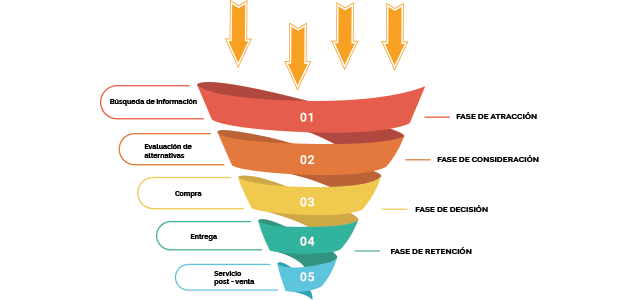
\includegraphics[width=13cm]{./Imagenes/canvas2}
	\end{center}
Lo que haremos es seleccionar aquellos canales online que nos van a permitir dar a conocer nuestro producto a nuestra audiencia objetivo para que terminen realizando la compra.\\
Por ejemplo, algunos de los canales que podremos utilizar serán:\\
\begin{itemize}
\item El posicionamiento SEO.
\item Publicidad SEM.
\item Redes Sociales.
\item Social Ads.
\item Estrategia de contenidos.
\item Email marketing.
\item Marketing de afiliación.
\end{itemize}
La clave estará en saber qué canal es mejor utilizar en cada una de las fases en las que se encuentre el cliente.


\subsubsection{Relaciones con los Clientes}
En la cuarta fase del método canvas deberás de establecer el tipo de relación que vas a tener con tus clientes.\\
Es decir, deberás de concretar qué tipo de relación vas a tener:\\
\begin{itemize}
\item Personal.
\item Automática
\item De autoservicio.
\item Pago único (Life time).
\item Pago mediante suscripción (mensual, trimestral, anual).

\end{itemize}

La clave se basa en pensar cómo hacer para que el cliente se sienta identificado con nuestra propuesta de valor para que permanezca a nuestro lado y no se vaya con la competencia.\\

Aquí está otro de los errores que cometen muchos emprendedores y que yo no quiero que cometas.\\

Muchas empresas únicamente se centran únicamente en conseguir y conseguir nuevos clientes sin cuidar a los clientes actuales.\\

Y no se dan cuenta de que cuesta más conseguir un nuevo cliente que retener a los clientes.\\

Por lo que será fundamental que en este apartado del modelo canvas definas cómo vas a mantener la relación con los clientes actuales.\\

\subsubsection{Fuentes de Ingresos}

Es en este punto del business model canvas donde tienes que reflejar las diferentes fuentes de ingresos que vas a conseguir. \\

Otro de los errores que cometen muchos emprendedores es empezar definiendo su modelo de negocio en base a las diferentes vías de ingresos que van a obtener.\\

Esto es un error porque la forma correcta de definir los ingresos de tu canvas es habiendo definido previamente los segmentos de clientes a los que te vas a dirigir.\\

Aquí deberás reflejar los ingresos en efectivo que vas a generar con cada segmento de clientes.\\

Para calcular esto, será fundamental que en el segundo apartado del lienzo de canvas (propuesta de valor) hayas empezado a analizar cuánto dinero van a estar dispuestos a pagar tus clientes por tus productos.\\

Además, deberás de definir cuáles van a ser las formas de pago que van a tener los clientes.\\

Principalmente, existen dos tipos de ingresos básicos\\
\begin{itemize}
\item Los pagos únicos
\item Los pagos periódicos
\end{itemize}
Y en función de estos dos tipos pueden darse varias formas de obtener ingresos:\\
\begin{itemize}
\item Alquiler. Por ejemplo, cuando alquilas un apartamento.
\item Cuota de servicio o uso. Por ejemplo las compañías de teléfono.
\item Cuota por suscripción. Sería el caso de Netflix o de un gimnasio.
\item Concesiones de licencia.
\item Comisiones de corretaje. Por ejemplo, las comisiones cobradas por un agente de bolsa.
\end{itemize}
\subsubsection{Recursos Clave}

Recapitulemos, hemos definido en la plantilla del modelo canvas quiénes son nuestros clientes, qué les vamos a ofrecer, cómo se lo vamos a ofrecer, qué tipo de relaciones vamos a mantener con ellos y cómo vamos a conseguir generar ingresos.\\

Ahora es cuando debemos de concretar los recursos claves que dispone la empresa para comunicar su propuesta de valor.\\

 Existen cuatro tipo de recursos clave:\\
\begin{itemize}
\item Humanos. Aquí deberás de tener en cuenta a todas las personas que necesitarás tener a disposición en tu organización.
\item Físicos. Deberás de concretar las instalaciones y maquinarias que tienes a disposición.
\item Intelectuales. Aquí entrarían las patentes, software, etc.
\item Económicos. Finalmente deberás incluir todos los recursos financieros de que dispones.
\end{itemize}
\subsubsection{Actividades Clave}

En este apartado de la matriz del modelo de negocio deberemos de tener en cuenta todas las actividades y procesos que serán necesarios para crear y ofrecer la propuesta de valor.\\

En su libro Osterwalder de Generación de Modelos de Negocio lo explica con un ejemplo muy sencillo “La actividad clave del fabricante de software Microsoft es el desarrollo de software.\\

También indica que las actividades clave relacionadas con las empresas están formadas por la producción, la venta y el soporte.\\

La actividad de producción va desde el diseño, la fabricación y el desarrollo de los productos y servicios de la empresa.\\

La venta engloba todas aquellas actividades vinculadas con la comunicación, promoción de la propuesta de valor de la empresa para hacerla llegar a sus segmentos de clientes.\\

Mientras que la parte de soporte incluye actividades como la contratación de personal o las tareas administrativas y contables.\\

Este punto en concreto del modelo de negocio canvas me gusta tratarlo desde la Cadena de Valor de Porter\\

Leyenda: Cadena de Valor de Porter\\

\begin{center}
	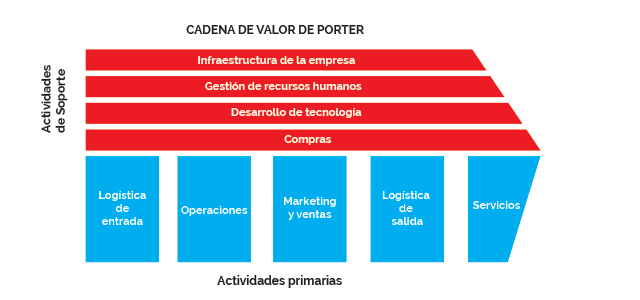
\includegraphics[width=13cm]{./Imagenes/ang1.png}
\end{center}

La cadena de valor de Porter sostiene que es un modelo que describe todas las actividades clave que lleva a cabo una empresa para generar valor (propuesta de valor) a su cliente final.\\

Por lo tanto, lo que deberías de hacer aquí es diferenciar entre las actividades de soporte y las primarias y clasificarla en orden de importancia para tu modelo de negocio.\\

\subsubsection{Asociaciones Clave}

Este es otro de los puntos esenciales del método canvas, aquí deberás de definir quiénes van a ser tus proveedores y tus socios estratégicos.\\

En este apartado me gustaría también citar al modelo de stakeholders que nombran en su libro Guerras y Navas\\

Leyenda: Stakeholders Guerras y Navas\\

\begin{center}
	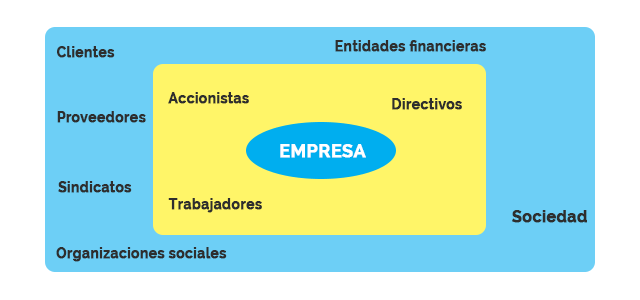
\includegraphics[width=13cm]{./Imagenes/ang2.png}
\end{center}
	
Los stakeholders o grupos de interés están formados por grupos de personas que tienen unos objetivos que están relacionados directa o indirectamente con la propia actividad de la empresa.\\

La clave aquí pasa por identificar los grupos más interesantes para la empresa y tratar de crear alianzas estratégicas con ellos.\\

\subsubsection{Estructura de Costes}

Finalmente, en el último módulo del business model canvas lo que deberemos de hacer es determinar la estructura de costes del canvas.\\

Esta estructura de costes estará formada principalmente por las actividades clave, los recursos clave y las asociaciones clave.\\

La estructura de costes de una empresa es fundamental para su viabilidad económica y es uno de los puntos más delicados del modelo de negocio canvas.\\

Tómate el tiempo que necesites en esta fase, porque la correcta imputación de los costes también puede marcar el éxito o el fracaso de un proyecto.\\



	%%
	%\linenumbers
	
	%% main text

\section{Diferencias}
Balanced Scorecard y Business model canvas son t\'ecnicas de análisis empresarial . Ambas t\'ecnicas son \'utiles para mejorar el desempeño organizacional. Pero sus aplicaciones son diferentes. Ambos se pueden usar junto con los indicadores clave de rendimiento para monitorear y mejorar el rendimiento de la organización
\begin{itemize}
\item Cuando usar Balanced Score Card.
   \\
    \\Se utilizan para monitorear el desempeño de la organización a lo largo del tiempo. Si se observa una caída estadística en la puntuación, la organización debe iniciar un cambio para detener la disminución del rendimiento. 
\item Cuando usar Business Model Canvas.
\\
      \\ Se puede usar como una herramienta de diagnóstico como una lente en el estado actual del negocio, especialmente en cantidades relativas de energía, tiempo y recursos que se invierten actualmente en diversas áreas. Si alguna de las áreas del modelo tiene un bajo rendimiento, la organización debe iniciar un cambio para mejorar el mismo.

\end{itemize}
%%
	
	%%
	%\linenumbers
	
	%% main text
\section{Conclusion}
   La gestión del desempeño contiene actividades que pueden garantizar que los objetivos se logren de manera consistente y eficaz. A través de Business Model Canvas, se le ofrece un concepto con el que puede describir, reflexionar e investigar el modelo de negocio de su organización. Un modelo de negocio se puede describir mejor sobre la base de nueve bloques de construcción básicos, que muestran la lógica de cómo una empresa quiere ganar dinero.
 El énfasis está en la implementación práctica del BSC y en la construcción de un tablero de instrumentos equilibrado, teniendo en cuenta no solo un tablero financiero, sino también la perspectiva del cliente, la perspectiva interna e innovadora. 
          

%%
	
	%%
	%\linenumbers
	
	%% main text


	\bibliographystyle{apalike} 	%ESTILO
	\bibliography{BIBLIOGRAFIA}		%ARCHIVO .bib
	
	%% The Appendices part is started with the command \appendix;
	%% appendix sections are then done as normal sections
	%% \appendix
	
	%% \section{}
	%% \label{}
	
	%% References
	%%
	%% Following citation commands can be used in the body text:
	%% Usage of \cite is as follows:
	%%   \cite{key}          ==>>  [#]
	%%   \cite[chap. 2]{key} ==>>  [#, chap. 2]
	%%   \citet{key}         ==>>  Author [#]
	
	%% References with bibTeX database:
	
	 \textcolor{blue}{\url{https://www.adaptiveus.com/balanced-scorecard-vs-business-model-canvas/}}
	 \textcolor{blue}{\url{   https://www.marketingandweb.es/emprendedores-2/que-es-el-modelo-canvas/}}

       
	%% Authors are advised to submit their bibtex database files. They are
	%% requested to list a bibtex style file in the manuscript if they do
	%% not want to use model1-num-names.bst.
	
	%% References without bibTeX database:
	
	% \begin{thebibliography}{00}
	
	%% \bibitem must have the following form:
	%%   \bibitem{key}...
	%%
	
	% \bibitem{}
	
	% \end{thebibliography}
	
	
\end{document}

%%
%% End of file `elsarticle-template-1-num.tex'.
